\documentclass[12pt]{article}
\usepackage[top=1in, bottom=1in, left=1in, right=1in]{geometry}

\usepackage{setspace}
\onehalfspacing

\usepackage{amssymb}
%% The amsthm package provides extended theorem environments
\usepackage{amsthm}
\usepackage{epsfig}
\usepackage{times}
\renewcommand{\ttdefault}{cmtt}
\usepackage{amsmath}
\usepackage{graphicx} % for graphics files
\usepackage{tabu}

% Draw figures yourself
\usepackage{tikz} 

% writing elements
\usepackage{mhchem}

% The float package HAS to load before hyperref
\usepackage{float} % for psuedocode formatting
\usepackage{xspace}

% from Denovo Methods Manual
\usepackage{mathrsfs}
\usepackage[mathcal]{euscript}
\usepackage{color}
\usepackage{array}

\usepackage[pdftex]{hyperref}
\usepackage[parfill]{parskip}

% math syntax
\newcommand{\nth}{n\ensuremath{^{\text{th}}} }
\newcommand{\ve}[1]{\ensuremath{\mathbf{#1}}}
\newcommand{\Macro}{\ensuremath{\Sigma}}
\newcommand{\rvec}{\ensuremath{\vec{r}}}
\newcommand{\vecr}{\ensuremath{\vec{r}}}
\newcommand{\omvec}{\ensuremath{\hat{\Omega}}}
\newcommand{\vOmega}{\ensuremath{\hat{\Omega}}}
\newcommand{\sigs}{\ensuremath{\Sigma_s(\rvec,E'\rightarrow E,\omvec'\rightarrow\omvec)}}
\newcommand{\el}{\ensuremath{\ell}}
\newcommand{\sigso}{\ensuremath{\Sigma_{s,0}}}
\newcommand{\sigsi}{\ensuremath{\Sigma_{s,1}}}
\newcommand{\ep}{\ensuremath{\varepsilon}}
%---------------------------------------------------------------------------
%---------------------------------------------------------------------------
\begin{document}
\begin{center}
{\bf NE 250, F15\\
November 22, 2015 
}
\end{center}

We've talked about how to discretize energy using the multigroup approximation and angle using $S_N$, $P_N$, or $SP_N$ for the transport equation. \\
This results in a set of ODEs and PDEs with space as the only variable.\\
In this class we're going to talk about options for handling that.
\begin{itemize}
\item Ray tracing: this is what we do in Monte Carlo and the integral form of the TE (solved with MOC). This allows us to represent ``exact" geometry.
\item There are two ways we can get equation sets with $\nabla^2$ operators: 
  \begin{itemize}
  \item the Diffusion equation. We can apply standard methods for this (learned in 150 I think, and definitely 155) or we can apply spherical harmonics in space, which can be manipulated to look a like a bunch of diffusion equations and we handle these as the regular DE.
  \item the even-odd parity TE (which we won't cover). This still has angular dependence but a diffusion-like operator so again we can use the same methods.
  \end{itemize}
\item We will look at the first order form ($\nabla$) here. 
\end{itemize}

\textbf{Spatial Discretization in Slab Geometry} (L\&M 3.3)\\
We'll start by thinking about the 1D, 1-group TE equation that has $S_N$ applied:
\begin{align*}
\mu_n \frac{d \psi_n}{dx} &+ \Sigma_t(x) \psi_n(x) = \sum_{l=0}^L (2l+1) P_l(\mu_n) \Sigma_{s,l}(x) \phi_l(x) + s_n(x)\\
\phi_l(x) &= \frac{1}{2}\sum_{n=1}^N w_n P_l(\mu_n) \psi_n(x)
\end{align*}
%
To deal with the spatial variable we divide space into a grid. The bins do not need to be evenly spaced.\\ 
%
\begin{center}
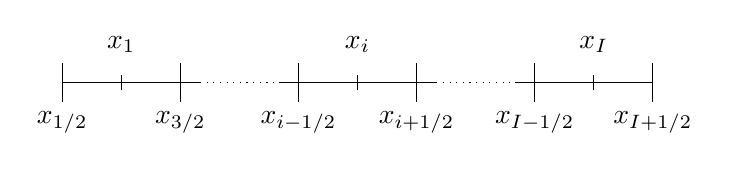
\begin{tikzpicture}
\draw (0,0)--(1.75,0);
\draw (0,-.25)--(0,.25);
\draw (1.5,-.25)--(1.5,.25);
\draw (0.75,-.1)--(0.75,.1);
\draw[dotted] (1.75,0)--(2.75,0);
\draw (2.75,0)--(4.75,0);
\draw[dotted] (4.75,0)--(5.75,0);
\draw (3,-.25)--(3,.25);
\draw (3.75,-.1)--(3.75,.1);
\draw (4.5,-.25)--(4.5,.25);
%\draw (5.25,-.1)--(5.25,.1);
%\draw (6,-.25)--(6,.25);
\draw (5.75,0)--(7.5,0);
\draw (6,-.25)--(6,.25);
\draw (6.75,-.1)--(6.75,.1);
\draw (7.5, -.25)--(7.5,.25);
\node[below] at (0,-.25) {$x_{1/2}$};
\node[above] at (0.75, .25) {$x_{1}$};
\node[below] at (1.5,-.25) {$x_{3/2}$};
\node[below] at (3,-.25) {$x_{i-1/2}$};
\node[below] at (4.5,-.25) {$x_{i+1/2}$};
%\node[below] at (6,-.25) {$x_{i+1}$};
\node[above] at (3.75, 0.25) {$x_{i}$};
%\node[above] at (5.25, 0.25) {$x_{i+1/2}$};
\node[below] at (6,-.25) {$x_{I-1/2}$};
\node[above] at (6.75, .25) {$x_{I}$};
\node[below] at (7.5,-.25) {$x_{I+1/2}$};
\end{tikzpicture}
\end{center}
%
In our derivation we will use both whole points (centers) and half points (edges), where whole points are halfway between the half points 
\[
x_{i} = \frac{x_{i+1/2} + x_{i-1/2}}{2} \:.
\]
We can think of these as computational cells, and the spatial values are centered around the whole points. Further, each cell is homogeneous. These two things mean
\[
\Sigma_{x,i} = \Sigma_x(x)\:, \quad x_{i-1/2} < x < x_{i+1/2} \:.
\]
Because we treat cross sections to be constant within each cell, we do well to align bin edges with material boundaries to the degree possible. We add cells where we need to in order to get the desired resolution.\\
We also define
\[
\Delta_i = x_{i+1/2} - x_{i-1/2}
\]
We also want to assign boundary conditions at the edges. For example:
\begin{align*}
\psi_{1/2,n} &= \psi_n(a_0)\:, \quad \forall n \text{ such that } \mu_n > 0 \\
\psi_{I+1/2,n} &= \psi_n(a_1)\:, \quad \forall n \text{ such that } \mu_n < 0 
\end{align*}
%
Next, we integrate the TE over each cell $i$:
\begin{align*}
\mu_n\bigl(&\psi_{i+1/2,n} - \psi_{i-1/2,n} \bigr) + \Delta_i \Sigma_{t,i} \psi_{i,n} = \Delta_i q_{i,n}\\
&\\
\psi_{i,n} &= \frac{1}{\Delta_i}\int_{x_{i-1/2}}^{x_{i+1/2}} \psi_n(x) dx \approx \psi_n(x_i) \quad \text{average flux across the cell}\\
q_{i,n} &\equiv \sum_{l=0}^L (2l+1) P_l(\mu_n) \Sigma_{s,l,i} \phi_{l,i} + s_{n,i}\:,
\end{align*}
where we used a midpoint rule for the integration.

This equation relates the cell-edge values and the cell-centered values.\\
To get an additional relationship between these values, we often use the ``diamond difference" relation.\\
To do this, we use a Taylor series in expansion cell $i$ about $x_i$ and evaluate the expansion at the half points:
\begin{align*}
\psi_n &= \psi_n(x_i) + (x - x_i)\frac{d\psi_n}{dx}|_{x_i} + \frac{1}{2}(x - x_i)^2 \frac{d^2 \psi_n}{dx^2}|_{x_i} + O(\Delta^3)\\
\psi_{n}(x_{i \pm 1/2}) &= \psi_n(x_i) + (x_{i \pm 1/2} - x_i) \frac{d\psi_n}{dx}|_{x_i} + \frac{(x_{i\pm 1/2} - x_i)^2}{2} \frac{d^2 \psi_n}{dx^2}|_{x_i} + O(\Delta^3)\\
\end{align*}
Next, we add the two half-point equations together:
\begin{align*}
\psi_{n, i+1/2} + \psi_{n, i-1/2} &= \psi_n(x_i) + \underbrace{(x_{i+1/2} + x_{i-1/2} - 2x_1)}_{0} \frac{d \psi_n}{dx}|_{x_i} + O(\Delta^2)\\
\psi_{n, i} &= \frac{1}{2}\bigl(\psi_{n,i+1/2} + \psi_{n,i-1/2}\bigr) + O(\Delta^2)
\end{align*}
and get the diamond difference relation.

\textbf{sweep pattern and boundary conditions}\\
We solve these equation in the direction of neutron flow by doing a mesh ``sweep". \\
We march through $i = 0, 1, \dots, I$ when $\mu_n > 0$. This is the direction of information transfer and maintains stability of our solution.\\
We march through $i = I, I-1, \dots, 0$ when $\mu_n < 0$ for the same reason.

Let's consider $\mu_n > 0$; we assume that we know $\psi_{n,i-1/2}$ (which works easily for vacuum of fixed incoming bcs) and solve for $\psi_{n,i}$ and $\psi_{n,i+1/2}$:
\[
\psi_{n,i} = \dfrac{\psi_{n, i-1/2} + \frac{\Delta_i q_{n,i}}{2 \mu_n}}{1 + \frac{\Delta_i \Sigma_{t,i}}{2 \mu_n}}
\]
We start at the left edge with $i=1$: $\psi_{n,1/2} = \psi(a_0)$.\\
Then we follow through $i>1$ using the continuity condition that  
\[
\psi_{n,i-1/2} = \psi_{n,(i-1)+1/2}\:.
\]
We get $\psi_{n,i+1/2}$ from the diamond difference relation:
\[
\psi_{n,i+1/2} = 2\psi_{n,i} - \psi_{n,i-1/2}\:.
\]
Note that we don't actually need $\psi_{n,i}$ after finding $\psi_{n,i+1/2}$ except for using it in computing the scattering and fission source, which actually requires the moments.  \\
To avoid storing $\psi_{n,i}$ we just build up and store the moments:
\[
\phi_{l,i} = \phi_{l,i} + \frac{1}{2}w_nP_l(\mu_n) \psi_{n,i}\:, \quad n = 1, \dots, N\:.
\]
We continue this process until we reach the right boundary.

Now let's consider coming back the other way, where $\psi_{n,i-1/2}$ is the outgoing flux. 
\begin{align*}
\psi_{n,I+1/2} &= \psi(a_1)\\
\psi_{n,i} &= \dfrac{\psi_{n, i+1/2} + \frac{\Delta_i q_{n,i}}{2 |\mu_n|}}{1 + \frac{\Delta_i \Sigma_{t,i}}{2 |\mu_n|}}\\
\psi_{n,i-1/2} &= 2\psi_{n,i} - \psi_{n,i+1/2}
\end{align*}
and we accumulate $\phi_{l,i}$ from the $\mu_n < 0$ contributions.

For reflecting, things are a little trickier. We need to map the outgoing flux moving one direction onto the incoming flux coming back the other direction. \\
If we assume that the right boundary is reflective and left is fixed, we
%
\begin{enumerate}
\item sweep left to right for $\mu_n > 0$;
\item use the previous process (determine $\psi_{n,i}$, accumulate $\phi_{l,i}$, compute $\psi_{n,i+1/2}$) until you reach the right boundary and solve for $\psi_{n,I+1/2}$;
\item determine $n'$ such that $\mu_{n'} = -\mu_n$ and set $\psi_{n',I+1/2} = \psi_{n,I+1/2}$;
\item sweep from right to left along $n'$.
\end{enumerate}
%
If you have reflective boundaries on both edges, then we start iterating using an initial guess for one of the boundary conditions. 

If we don't have secondary neutron production from fission or scattering (pure absorption and/or only downscattering), then one mesh sweep completely solves the problem. \\
This is equivalent to solving a lower-triangular matrix equation, $\mathbf{L}\mathbf{\psi} = \mathbf{q}$ (which we get by ordering the solve in the direction of neutron travel).

NOTE: we don't actually create and store this matrix, however. Because we only deal with the coefficients that couple the center and half points, we don't actually need the matrix.   This allows us to avoid memory restrictions for complex problems. \\
When we have one reflecting boundary, we can write our matrix equations as $\mathbf{L}\mathbf{\psi}^{m+1} = \mathbf{q}^m$.\\
When we have two reflecting boundaries, we get $\mathbf{L}\mathbf{\psi}^{m+1} = \mathbf{q}^m + \mathbf{U}\mathbf{\psi}^{m}$, where $\mathbf{U}$ is a strictly upper triangular matrix that operates on the flux from the previous iterate that has been ``reflected" off of the boundary.

\textbf{Local Truncation Error}\\




\textbf{Spatial Discretization in Multi-D} (L\&M 4.3)\\
\begin{minipage}{0.5\textwidth}
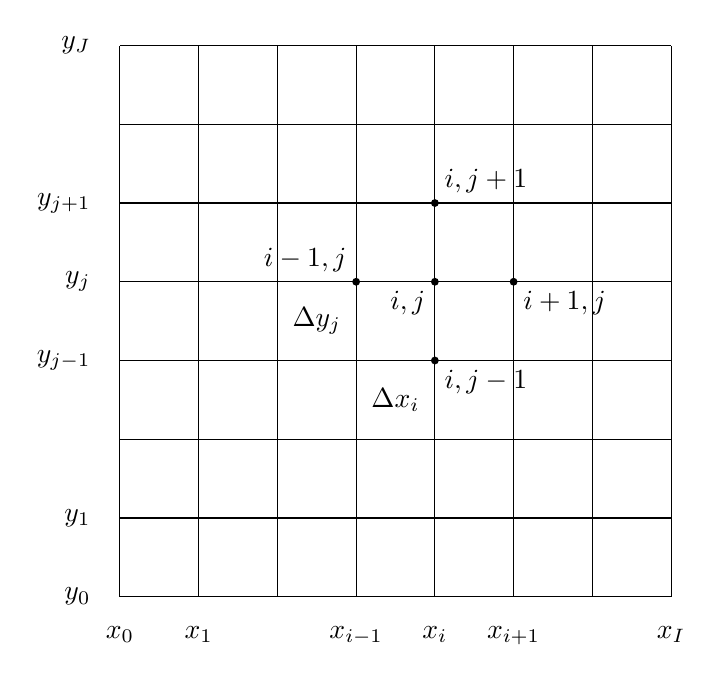
\begin{tikzpicture}
\draw (0,0)--(0,7);
\draw (1,0)--(1,7);
\draw (2,0)--(2,7);
\draw (3,0)--(3,7);
\draw (4,0)--(4,7);
\draw (5,0)--(5,7);
\draw (6,0)--(6,7);
\draw (7,0)--(7,7);
\node[below] at (0,-.25) {$x_0$};
\node[below] at (1,-.25) {$x_1$};
\node[below] at (3,-.25) {$x_{i-1}$};
%\node[above] at (3.5, .25) {$x_{i-1/2}$};
\node[below] at (4,-.25) {$x_i$};
%\node[above] at (4.5, .25) {$x_{i+1/2}$};
\node[below] at (5,-.25) {$x_{i+1}$};
\node[below] at (7,-.25) {$x_I$};
\node at (3.5, 2.5) {$\Delta x_i$};
% begin y
\draw (0,0)--(7,0);
\draw (0,1)--(7,1);
\draw (0,2)--(7,2);
\draw (0,3)--(7,3);
\draw (0,4)--(7,4);
\draw (0,5)--(7,5);
\draw (0,6)--(7,6);
\draw (0,7)--(7,7);
\node[left] at (-.25, 0) {$y_0$};
\node[left] at (-.25,1) {$y_1$};
\node[left] at (-.25,3) {$y_{j-1}$};
\node[left] at (-.25,4) {$y_j$};
\node[left] at (-.25,5) {$y_{j+1}$};
\node[left] at (-.25,7) {$y_J$};
  \node at (2.5,3.5) {$\Delta y_j$};
% labels
\node at (4,4) [circle,fill=black,scale=0.3] {};
\node[below left] at (4,4) {$i,j$};
\node at (5,4) [circle,fill=black,scale=0.3] {};
\node[below right] at (5,4) {$i+1,j$};
\node at (3,4) [circle,fill=black,scale=0.3] {};
\node[above left] at (3,4) {$i-1,j$};
\node at (4,5) [circle,fill=black,scale=0.3] {};
\node[above right] at (4,5) {$i,j+1$};
\node at (4,3) [circle,fill=black,scale=0.3] {};
\node[below right] at (4,3) {$i,j-1$};
\end{tikzpicture}
\end{minipage} \hfill
%
\begin{minipage}{0.5\textwidth}
  \[u(x_i,y_j) = u_{i,j} \qquad u(x_{i+1},y_j) = u_{i+1,j}\]
  \begin{align}
  \frac{\partial^2 u_{i,j}}{\partial x^2} = \frac{\partial}{\partial x}\bigl(\frac{\partial u_{i,j}}{\partial x}\bigr) =
\frac{u_{i-1,j} - 2u_{i,j} + u_{i+1,j}}{\Delta x_i^2} \nonumber \\
%
  \frac{\partial^2 u_{i,j}}{\partial y^2} = \frac{\partial}{\partial y}\bigl(\frac{\partial u_{i,j}}{\partial y}\bigr) =
\frac{u_{i,j-1} - 2u_{i,j} + u_{i,j+1}}{\Delta y_j^2} \nonumber
\end{align}
\end{minipage}

- boundary conditions and sweeping  pattern\\
- quick mention of other spatial methods and their properties


rest of course (3 classes left):\\
- M, 11/23: equation solution procedures (inner iteration, outer iteration, eigenvalue iteration, convergence); one basic solver of each type (SI, GS, PI)\\ 
- M, 11/30: example of research into a different solver for each type (block Krylov, RQI)
- W, 12/02: choice preconditioners? computing architectures? some topic we skipped? Last half of class will be feedback and discussion of class.




\end{document}